\chapter{Evaluasi Kurikulum dan Tracer Study}

\renewcommand{\arraystretch}{1.3}
\setstretch{1.15}

\section{Evaluasi Kurikulum}

Program Studi D4 Teknik Informatika telah mengadakan review dan evaluasi kurikulum yang melibatkan alumni yang telah bekerja di berbagai industri, pihak industri yang mempekerjakan alumni, serta dosen-dosen program studi. Prodi D4 Teknik Informatika mengadakan beberapa Forum Group Discussion (FGD) untuk mendapatkan masukan yang komprehensif terhadap pengembangan kurikulum.

\subsection{Saran dan Masukan terkait Profil Lulusan}

Profil lulusan yang sudah ada sebagian besar telah mencakup kebutuhan industri. Namun terdapat beberapa profil atau kompetensi tambahan yang belum tercakup, antara lain:

\begin{enumerate}
\item Quality Assurance dan Software Tester, baik manual maupun otomasi.
\item Technical Writer.
\item System Analyst.
\item Data Integrator: mengelola, mengolah, dan menampilkan seluruh data perusahaan ke sebuah dashboard.
\item System Implementator: implementasi produk dari klien.
\item DevOps Engineer: menyiapkan infrastruktur, cloud server, dan skrip otomasi.
\item ERP background: setup modul ERP berbayar maupun open source.
\end{enumerate}

Perkembangan industri yang perlu diadaptasi dalam kurikulum mencakup:
\begin{itemize}
\item Cloud service: AWS, Alibaba, dan DevOps.
\item Data Integration menggunakan konsep ETL dan Spark, serta pengenalan NoSQL.
\item Quality Assurance Engineering dan Tester Engineering.
\item Business Analyst dan Scrum Master.
\item Design Pattern dan praktik rekayasa seperti TDD.
\end{itemize}

\subsection{Saran dan Masukan berdasarkan Kuesioner Dosen}

Kuesioner evaluasi kurikulum disebarkan kepada dosen Jurusan Teknologi Informasi Politeknik Negeri Malang. Jumlah total partisipan yang mengisi kuesioner adalah 21 dosen.

\subsubsection{Profil Lulusan dari Program Studi D-IV Teknik Informatika}

Berdasarkan data alumni, profil lulusan yang paling banyak digeluti adalah sebagai berikut:

\begin{center}
\begin{tabular}{L{9cm}C{3cm}}
\toprule
Profil Lulusan & Jumlah Alumni \\
\midrule
Software Engineer & 21 \\
Database Administrator & 21 \\
Web Engineer / Web Administrator & 19 \\
Developer Game & 18 \\
Network Engineer / Data Communication Engineer & 17 \\
IT Entrepreneur & 17 \\
System Programmer & 17 \\
IT Technical Support & 14 \\
Software Tester & 13 \\
Intelligence System Developer & 12 \\
IT Project Manager & 10 \\
\bottomrule
\end{tabular}
\end{center}

Deskripsi masing-masing profil lulusan:

\begin{description}
\item[Software Engineer] Menerapkan pendekatan sistematis dalam pengembangan, pengoperasian, dan pemeliharaan perangkat lunak.
\item[Database Administrator] Membuat rancangan basis data, mengimplementasikan rancangan tersebut, serta melakukan instalasi, konfigurasi, upgrade, adaptasi, pemantauan, dan pemeliharaan basis data dalam suatu organisasi.
\item[Web Engineer / Web Administrator] Merencanakan, mengembangkan, dan memelihara website.
\item[Developer Game] Mengembangkan perangkat lunak permainan multimedia.
\item[Network Engineer / Data Communication Engineer] Merancang arsitektur jaringan komputer, termasuk perawatan dan manajemennya di perusahaan atau organisasi.
\item[IT Entrepreneur] Membangun dan mengembangkan usaha mandiri berbasis teknologi komputer yang memberikan dampak kesejahteraan bagi masyarakat.
\item[System Programmer] Menganalisis, merancang, mengembangkan, dan mengimplementasikan solusi perangkat lunak pada platform mobile dan web.
\item[IT Technical Support] Melakukan administrasi, perbaikan, dan perawatan peralatan dan infrastruktur IT baik secara software maupun hardware.
\item[Software Tester] Mengevaluasi dan memastikan bahwa perangkat lunak berjalan dengan benar sesuai dengan yang ditentukan.
\item[Intelligence System Developer] Mengembangkan sistem yang dapat melakukan pembelajaran dan penalaran berdasarkan pengetahuan yang sesuai dengan masalah yang dihadapi.
\item[IT Project Manager] Membuat rencana dan proses untuk memantau perkembangan proyek serta mengelola tim.
\end{description}

\subsubsection{Kompetensi yang Harus Dimiliki Lulusan}

Berikut kompetensi utama yang diusulkan harus dimiliki lulusan Program Studi D4 Teknik Informatika:

\begin{center}
\begin{tabular}{L{10cm}C{2.5cm}}
\toprule
Kompetensi & Jumlah \\
\midrule
Pengembangan aplikasi mobile dan layanan berbasis web & 20 \\
Kemampuan membuat perangkat lunak untuk menyelesaikan masalah & 19 \\
Teknik-teknik pemrograman komputer, sistem komputer, sistem jaringan komputer & 18 \\
Mampu mendesain, membuat, dan mengelola Database & 18 \\
Pengembangan game (skenario, algoritma, pemrograman, grafis, multimedia) & 17 \\
Technopreneurship & 17 \\
Mampu membuat program berbasis web dengan baik & 17 \\
Mampu mengimplementasikan dan mengelola jaringan komputer & 16 \\
Mampu membuat program komputer dengan baik & 14 \\
Full stack developer di bidang mobile/web programming & 14 \\
Mampu menggunakan aplikasi perkantoran sederhana maupun rumit & 11 \\
\bottomrule
\end{tabular}
\end{center}

\subsubsection{Mata Kuliah yang Perlu Ditambahkan}

Sebanyak 12 dosen memilih bahwa perlu ditambahkan mata kuliah baru pada program studi D-IV Teknik Informatika:

\begin{center}
\begin{tabular}{L{9cm}C{3cm}}
\toprule
Nama Mata Kuliah & Jumlah Pengusul \\
\midrule
Pemrograman Mobile Lanjut & 3 \\
Manajemen Jaringan Komputer & 2 \\
Web Front End, Web Back End, UI dan UX & 2 \\
Multimedia Coding / Pengkodean Multimedia & 1 \\
DevOps & 1 \\
Kriptografi & 1 \\
Rancangan Analisis Algoritma & 1 \\
Cyber Security dan Blockchain & 1 \\
Desain Infrastruktur TI & 1 \\
Manajemen Basis Data Modern (NoSQL, master-slave, replikasi) & 1 \\
Manajemen dan Keamanan Jaringan Komputer & 1 \\
Materi Git pada MK Teknik Dokumentasi & 1 \\
\bottomrule
\end{tabular}
\end{center}

\subsubsection{Mata Kuliah yang Perlu Dihapus atau Digabung}

Sebanyak 10 dosen memilih bahwa terdapat mata kuliah yang perlu dihapus atau dikurangi:

\begin{center}
\begin{tabular}{L{5cm}L{8cm}}
\toprule
Mata Kuliah & Saran \\
\midrule
Sistem Manajemen Basis Data & Digabung dengan Basis Data Lanjut \\
Pengantar Teknologi Informasi & Digabung ke Kecerdasan Buatan \\
Proyek & Proyek 1 + Proyek 2 + Proyek 3 dilebur menjadi satu mata kuliah \\
Komputasi Multimedia & Diganti dengan Virtual Reality \\
E-business & Digabung dengan Metodologi Penelitian \\
Kapita Selekta & Digabung dengan mata kuliah proyek \\
Teknik Dokumentasi & Digabung dengan Basis Data Lanjut (function, trigger, administrasi DB) \\
Pemrograman Web Framework & -- \\
Aplikasi Komputer Perkantoran & -- \\
Ilmu Komunikasi dan Organisasi & -- \\
\bottomrule
\end{tabular}
\end{center}

\subsubsection{Saran Umum dari Dosen}

\begin{enumerate}
\item Diskusi rutin untuk pengembangan kurikulum.
\item Jika diadakan peminatan, sebaiknya ditentukan secara holistik melalui kecenderungan nilai, isian form peminatan, dan tes peminatan.
\item Perlu dianalisa capaian pembelajaran tiap mata kuliah.
\item Diperlukan adanya konsentrasi (peminatan) pada kurikulum dan penambahan mata kuliah pilihan sesuai peminatan.
\item Kurikulum harus selalu diperbarui sesuai dengan tuntutan industri.
\item Proyek dapat dihapus/digabung/dikurangi; bisa diganti mata kuliah Manajemen Jaringan agar lebih mendukung mata kuliah IoT.
\item Kurikulum pendidikan vokasi perlu mengarah pada penciptaan kompetensi/skill yang tersertifikasi sehingga lulusan memiliki nilai tambah tidak hanya ijazah.
\item Mahasiswa di pertengahan hingga akhir semester sebaiknya diberikan pilihan konsentrasi, karena DU/DI lebih cenderung merekrut \textit{specialist} daripada \textit{generalist}.
\item Pada semester awal, porsi mata kuliah teknis sebaiknya sekitar 70\%.
\item Melibatkan industri untuk mereview rancangan kurikulum secara berkala.
\end{enumerate}

\subsection{Saran dan Masukan berdasarkan FGD dengan Industri}

Pada hari Jumat, 4 Desember 2020, telah dilaksanakan \textit{Focus Group Discussion} (FGD) untuk mendapatkan masukan dari industri terhadap kurikulum Program Studi D4 Teknik Informatika, dengan menghadirkan narasumber:

\begin{tabular}{L{3cm}L{9.5cm}}
Nama & : Martin Fatnuriyah \\
Industri & : The Edge Property, Pte. Ltd \\
Jabatan & : Technical Director \\
\end{tabular}

Poin-poin evaluasi dan rekomendasi dari FGD:

\begin{enumerate}
\item Posisi talent di The Edge Property terbagi menjadi: \textit{front end developer}, \textit{back end developer}, \textit{quality assurance}, \textit{data engineer}, dan \textit{full stack developer}.
\item Lulusan Polinema dinilai memiliki kelebihan di sisi hard skill dan soft skill, sehingga beberapa alumni berhasil menduduki posisi team lead dari fresh graduate.
\item Proses seleksi mencakup: initial interview, online assessment (algoritma dan analitik), project assessment, dan final interview (time management dan project management).
\item Data engineer berbeda dengan Database Administrator: data engineer menguasai pemrosesan data, representasi data, dan visualisasi data untuk data analitik.
\item Profil Quality Assurance belum ter-cover di perguruan tinggi; QA bertugas menentukan apakah produk bisa di-\textit{release} berdasarkan test plan.
\item Teknologi yang digunakan:
  \begin{itemize}
  \item Backend: Node.js, Python, PHP Laravel, teknologi \textit{micro service}.
  \item Frontend: Angular.js, Next.js, native JavaScript, jQuery.
  \item Fullstack: diharapkan mampu menguasai backend dan frontend.
  \item Database: MySQL dan NoSQL.
  \end{itemize}
\item Soft skill yang harus dipersiapkan: \textit{communication skills}, \textit{presentation skills}, dan \textit{leadership skills}.
\item Kekurangan yang sering ditemui: kurang percaya diri saat berkomunikasi dalam bahasa Inggris dan lintas divisi, serta kurang berani menolak tugas-tugas yang tidak sesuai.
\end{enumerate}

\section{Tracer Study Alumni D4 Teknik Informatika}

Tracer study dilakukan untuk mengetahui profil dan keterserapan lulusan Program Studi D4 Teknik Informatika di dunia kerja. Data pada bagian ini bersumber dari tracer study resmi yang dilaksanakan terhadap alumni lulusan tahun 2022, 2023, dan 2024, dengan total \textbf{344 responden}.

\begin{center}
\begin{tabular}{L{6cm}C{4cm}}
\toprule
Tahun Lulus & Jumlah Responden \\
\midrule
2022 & 102 \\
2023 & 127 \\
2024 & 115 \\
\midrule
Total & 344 \\
\bottomrule
\end{tabular}
\end{center}

\subsection{Masa Tunggu Memperoleh Pekerjaan}

Sebagian besar alumni memperoleh pekerjaan dalam waktu singkat setelah lulus: 41,0\% telah bekerja sebelum atau segera setelah lulus, 59,6\% telah bekerja dalam waktu 3 bulan, dan 77,3\% telah bekerja dalam waktu 6 bulan. Hanya 19 alumni (5,5\%) yang membutuhkan waktu lebih dari 12 bulan untuk memperoleh pekerjaan pertama.

\begin{center}
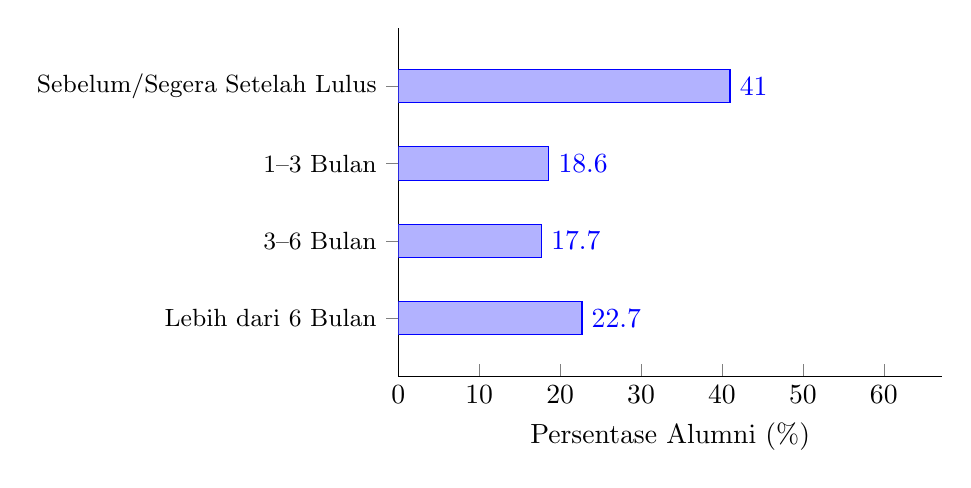
\begin{tikzpicture}
\begin{axis}[
  xbar,
  bar width=12pt,
  width=0.7\linewidth,
  height=6cm,
  xlabel={Persentase Alumni (\%)},
  symbolic y coords={Lebih dari 6 Bulan,3--6 Bulan,1--3 Bulan,Sebelum/Segera Setelah Lulus},
  ytick=data,
  nodes near coords,
  nodes near coords align={horizontal},
  xmin=0, xmax=60,
  enlarge x limits={upper, value=0.12},
  enlarge y limits=0.25,
  y tick label style={font=\small},
  axis lines*=left,
]
\addplot coordinates {(41.0,Sebelum/Segera Setelah Lulus) (18.6,1--3 Bulan) (17.7,3--6 Bulan) (22.7,Lebih dari 6 Bulan)};
\end{axis}
\end{tikzpicture}
\end{center}

\subsection{Jenis dan Status Pekerjaan}

Mayoritas alumni bekerja sebagai karyawan swasta (71,2\%). Sebanyak 55,2\% alumni menyatakan pekerjaannya sesuai dengan bidang studi, sementara 44,8\% bekerja di luar bidang studi.

\begin{center}
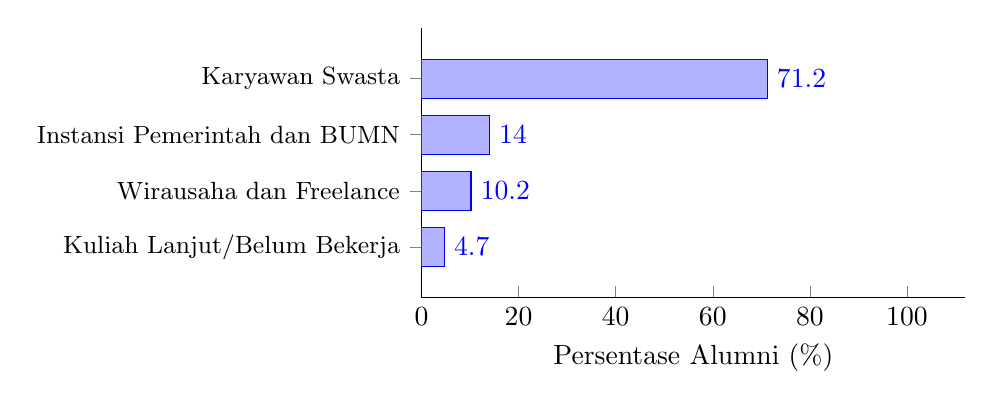
\begin{tikzpicture}
\begin{axis}[
  xbar,
  bar width=14pt,
  width=0.7\linewidth,
  height=5cm,
  xlabel={Persentase Alumni (\%)},
  symbolic y coords={Kuliah Lanjut/Belum Bekerja,Wirausaha dan Freelance,Instansi Pemerintah dan BUMN,Karyawan Swasta},
  ytick=data,
  nodes near coords,
  nodes near coords align={horizontal},
  xmin=0, xmax=100,
  enlarge x limits={upper, value=0.12},
  enlarge y limits=0.3,
  y tick label style={font=\small},
  axis lines*=left,
]
\addplot coordinates {(71.2,Karyawan Swasta) (14.0,Instansi Pemerintah dan BUMN) (10.2,Wirausaha dan Freelance) (4.7,Kuliah Lanjut/Belum Bekerja)};
\end{axis}
\end{tikzpicture}
\end{center}

\begin{center}
\begin{tabular}{L{9cm}C{2cm}C{2.5cm}}
\toprule
Jenis Pekerjaan & Jumlah & Persentase \\
\midrule
Karyawan Swasta & 245 & 71,2\% \\
Kontrak Institusi Pemerintah & 27 & 7,8\% \\
Wirausaha & 21 & 6,1\% \\
BUMN & 17 & 4,9\% \\
Melanjutkan Kuliah & 15 & 4,4\% \\
Freelance / Jasa Lepas & 14 & 4,1\% \\
Pegawai Negeri Sipil & 3 & 0,9\% \\
Tentara Nasional Indonesia & 1 & 0,3\% \\
Belum Bekerja & 1 & 0,3\% \\
\midrule
Total & 344 & 100\% \\
\bottomrule
\end{tabular}
\end{center}

\subsection{Tingkat Pendapatan}

Dari 344 responden, 261 alumni (75,9\%) mengisi data pendapatan bulanan. Rata-rata pendapatan alumni berada pada kisaran Rp4,65 juta per bulan, dengan nilai tengah (median) Rp3,7 juta per bulan.

\begin{center}
\begin{tabular}{L{7cm}C{4cm}}
\toprule
Indikator & Nilai \\
\midrule
Rata-rata pendapatan bulanan & Rp4.650.920 \\
Median pendapatan bulanan & Rp3.700.000 \\
Jumlah responden mengisi & 261 dari 344 \\
\bottomrule
\end{tabular}
\end{center}

\subsection{Sebaran Wilayah dan Bidang Kerja}

Mayoritas alumni bekerja di Provinsi Jawa Timur (66,9\%) dan DKI Jakarta (18,3\%), dengan sisanya tersebar di berbagai provinsi di Indonesia.

\begin{center}
\begin{tabular}{L{7cm}C{2cm}C{2.5cm}}
\toprule
Provinsi & Jumlah & Persentase \\
\midrule
Jawa Timur & 230 & 66,9\% \\
DKI Jakarta & 63 & 18,3\% \\
Jawa Barat & 11 & 3,2\% \\
DI Yogyakarta & 7 & 2,0\% \\
Bali & 6 & 1,7\% \\
Kalimantan Timur & 5 & 1,5\% \\
Banten & 4 & 1,2\% \\
Nusa Tenggara Barat & 4 & 1,2\% \\
Lainnya (10 provinsi lain) & 14 & 4,1\% \\
\midrule
Total & 344 & 100\% \\
\bottomrule
\end{tabular}
\end{center}

Alumni tersebar pada 305 perusahaan/instansi yang berbeda (dari 344 responden yang bekerja), dengan bidang kerja terbanyak pada sektor teknologi informasi, pendidikan, dan perbankan/keuangan. Sebaran ini menunjukkan keterserapan lulusan yang luas lintas industri, tidak terkonsentrasi pada segelintir pemberi kerja.

\begin{center}
\begin{tabular}{L{7cm}C{2cm}C{2.5cm}}
\toprule
Bidang Kerja & Jumlah & Persentase \\
\midrule
Teknologi Informasi & 34 & 9,9\% \\
Pendidikan & 26 & 7,6\% \\
Tidak Diisi & 21 & 6,1\% \\
Software / Software House & 19 & 5,5\% \\
Perbankan / Keuangan & 11 & 3,2\% \\
Manufaktur & 9 & 2,6\% \\
Telekomunikasi & 5 & 1,5\% \\
Perdagangan & 5 & 1,5\% \\
Lainnya (bidang lain, tersebar) & 214 & 62,2\% \\
\midrule
Total & 344 & 100\% \\
\bottomrule
\end{tabular}
\end{center}

\subsection{Catatan Historis: Aspek Kompetensi Lulusan (Survei 2020)}

\reviewfrompdf{Survei tracer study 2022--2024 di atas tidak mencakup penilaian aspek kompetensi (hard skill/soft skill) lulusan. Poin-poin berikut adalah temuan kualitatif dari tracer study kurikulum 2020 (alumni lulusan 2017/2018--2019/2020, 199 partisipan) dan dipertahankan sebagai catatan historis, bukan data final.}

\begin{itemize}
\item \textbf{Aspek keunggulan lulusan (hard skill):} kemampuan analitis (80\%) dan kemampuan desain serta implementasi solusi.
\item \textbf{Aspek keunggulan lulusan (soft skill):} norma, integritas, disiplin, tanggung jawab, dan efisiensi.
\item \textbf{Aspek kelemahan lulusan:} Bahasa Inggris (15,08\%), komunikasi (4,01\%), dan kerja sama tim (3,02\%).
\end{itemize}

\renewcommand{\arraystretch}{1.08}
\setstretch{1.08}
